% composite.tex
%
\section{Chart::Composite}
\name{Chart::Composite}
\file{Composite.pm}
\requires{Chart::Base, GD, Carp, FileHandle}
\begin{Description} \class{Composite} is a subclass of \class{Chart::Base}.\\
The class \class{Composite} creates a two component chart 
with two types of charts which are layed 
one above each other.
Therefore, two similiar chart types may have a conflict in the printout.
For example, you can create a two component chart with bars and lines. 
Just set the option 'composite\_info'! 
A composite chart doesn't make sense with all types of chart. 
But it works pretty good with Lines, Points, LinesPoints and Bars.
\end{Description}

\parindent 0pt{\large Example:}
\begin{figure}[h]
	\begin{center}
		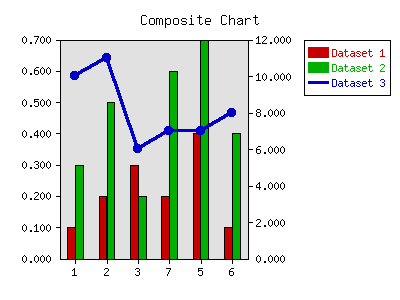
\includegraphics[scale=0.6]{composite_f.png}
	\end{center}
	\caption{Composite chart}
	\label{fig:composite}
\end{figure}
\begin{verbatim}
use Chart::Composite;

$g = Chart::Composite->new;

$g->add_dataset (1 , 2, 3, 4, 5, 6);
$g->add_dataset (0.1, 0.2, 0.3, 0.2, 0.4, 0.1);
$g->add_dataset (0.3, 0.5, 0.2, 0.6, 0.7, 0.4);
$g->add_dataset (10, 11, 6, 7, 7, 8);

$g->set('title' => 'Composite Chart',
        'composite_info' => [ ['Bars', [1,2]],
                               ['LinesPoints', [3]] ] );
$g->set( 'include_zero' => 'true');

$g->png("composite.png");
\end{verbatim}

\begin{Constructor} 
An instance of a Composite object can be created with the constructor new():
\begin{quote}
\parindent 0pt
\fett{\$obj = Chart::Composite->new();}\\
\fett{\$obj = Chart::Composite->new(\parameter{width}, \parameter{height});}
\end{quote}
If \textit{new()} has no arguments, 
the constructor returns an image with the size 300x400 pixels. 
If \textit{new()} has two arguments \parameter{width} and \parameter{height}, 
it returns an image of the desired size.
\end{Constructor}

\Methods
All universally valid methods, see page \pageref{methods}: \class{Chart::Base}. \\

\Attributes
All universal valid options, see page \pageref{options}. 

The following options are also available:
\begin{description}
\item['composite\_info'] This option is only used for composite charts.  
      It contains the information about which types to use for the two component charts, 
      and which datasets belong to which component chart. 
      It should be a reference to an array of array references, 
      containing information like the following\\
      \$obj->set ('composite\_info' => [ ['Bars', [1,2]],  ['Lines', [3,4] ] ]);\\
\\
      This example would set the two component charts to be a bar chart and a line chart. 
      It would use the first two data sets for the bar chart
      (note that the numbering starts at 1, 
      not zero like most of the other numbered things in Chart), 
      and the second two data sets for the line chart. The default is undef.\\
      \\
      NB. Chart::Composite can only do two component charts.
      
\item['min\_val1', 'min\_val2'] Only for composite charts, 
     these options specify the minimum y-value for the first and second components
     respectively. Both default to undef.

\item['max\_val1', 'max\_val2'] Only for composite charts, 
     these options specify the maximum y-value for the first and second components
     respectively. Both default to undef.

\item['y\_ticks1', 'y\_ticks2'] The number of y ticks to use on the first 
     and second y-axis on a composite chart.  
     Please note that if you just set the 'y\_ticks' option, 
     both axes will use that number of y ticks. Both default to undef.

\item['brush\_size1', 'brush\_size2'] If using compositite charts having
     'brush\_size' as their attribute you can define the size of the brush
     individually. Default is 6.
     
\item['f\_y\_tick1', 'f\_y\_tick2'] Needs a reference to a function which uses the y-tick
     labels for the first and second y-axis. 
     The result of this function reformats the labels as a string. For instance\\
     \\
     \$obj -> set ('f\_y\_tick1') => \verb|\|\&formatter1 ;\\
     \$obj -> set ('f\_y\_tick2') => \verb|\|\&formatter2 ;\\

\item['same\_y\_axes'] Forces both component charts in a composite chart 
     to use the same maximum and minimum y-values if set to 'true'. 
     This helps to keep the composite charts from being too confusing. Default is undef.
     
\item['legend\_example\_height'] Only for composite charts. These option changes the thickness
     of the lines in the legend. If 'legend\_example\_height' ist set to 'true'the 
     thickness of all 'legend-lines' can be changed. Default is false.\\
     \\
     \$obj -> set ('legend\_example\_height'    => 'true');\\
     \$obj -> set ('legend\_example\_height0'   => '3');\\
     \$obj -> set ('legned\_example\_height1..4'=> '10');\\
     \\
     This example would set the thickness of the first line in the legend to 3, and the 
     thickness of the following 4 lines to 10. The Defaultvalues of the individual datasets
     (use the same order as in 'composite\_info') are one, which means a 'normal' line
     is drawn. It is not possible to change a 'legend\_example\_height\#'(\# means a                 datasetnumber)which was once defined. The first value remains.            
                      
\end{description}
